\appendix
\chapter{Онтологические модели системы электронного обучения} \label{APP_A}

 \section{Онтологическая модель учебных материалов}\label{APP_A_EDU}

\begin{figure} [h] 
  \center
  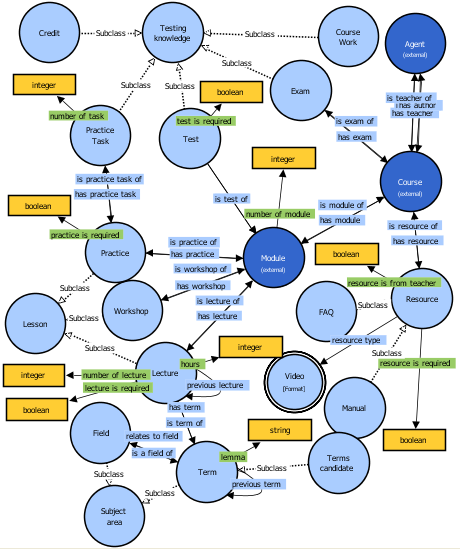
\includegraphics [scale=0.95] {ontology_edu}
  \caption{Основные классы и свойства онтологии учебных материалов.} 
  \label{img:ontology_edu}  
\end{figure}

\clearpage

 \section{Пример связывания объектов онтологии учебных материалов}\label{APP_A_EXMPL}

\begin{figure} [h] 
  \center
  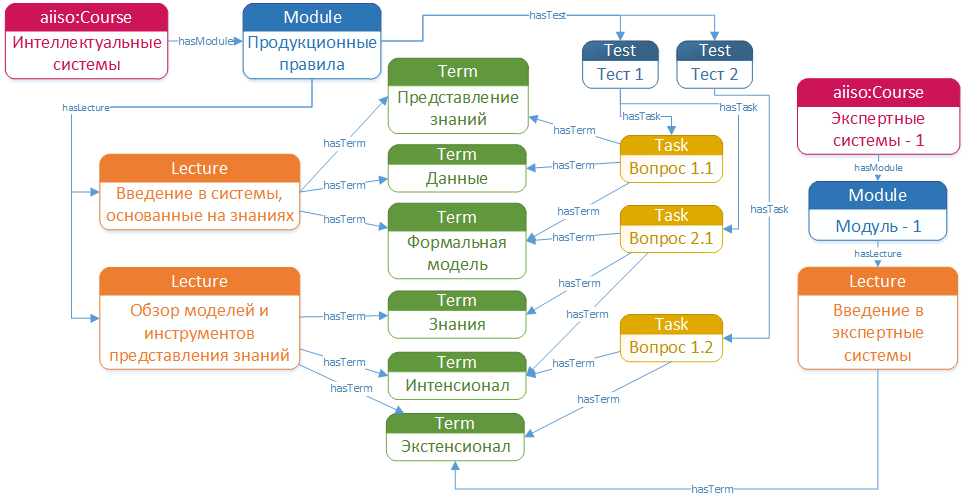
\includegraphics [scale=0.65] {ontology_edu_example_full}
  \caption{Пример связывания объектов онтологии учебных материалов.} 
  \label{img:ontology_edu_example_full}  
\end{figure}

\clearpage

 \section{Онтологическая модель тестов}\label{APP_A_TEST}

\begin{figure} [h] 
  \center
  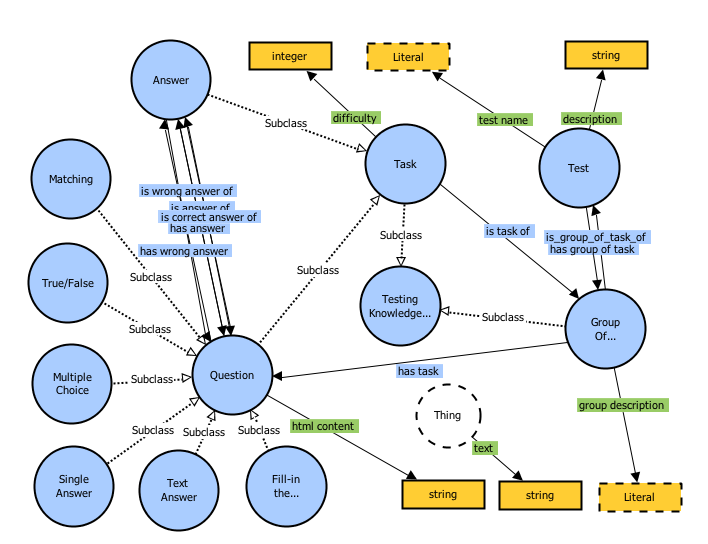
\includegraphics [scale=0.65] {ontology_test}
  \caption{Основные классы и свойства онтологии тестов.} 
  \label{img:ontology_test}  
\end{figure}

\clearpage

 \section{Онтологическая модель действий студента в системе электронного обучения}\label{APP_A_ACTION}

\begin{figure} [h] 
  \center
  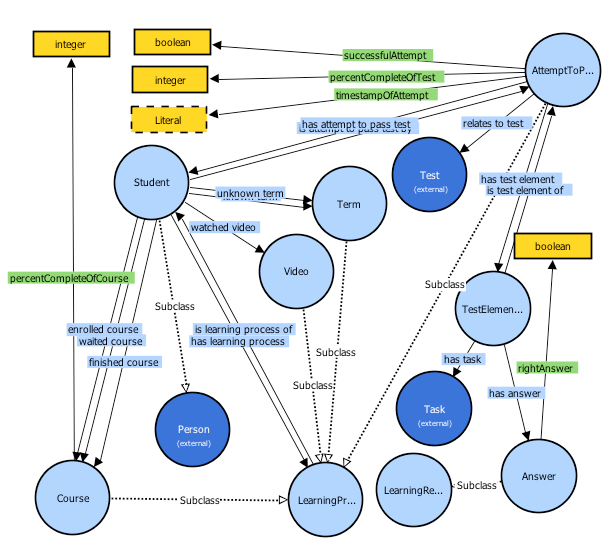
\includegraphics [scale=0.75] {ontology_action}
  \caption{Основные классы и свойства онтологии действий студента в системе электронного обучения.} 
  \label{img:ontology_action}  
\end{figure}

\clearpage

 \section{Онтологическая модель оценки знаний студентов}\label{APP_A_KNOW}

\begin{figure} [h] 
  \center
  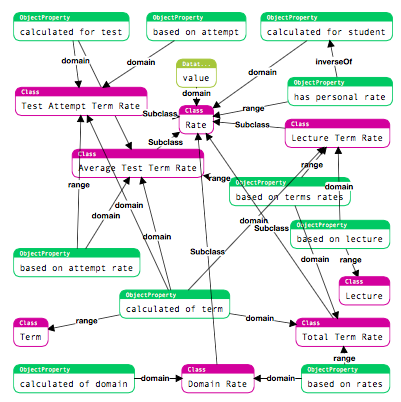
\includegraphics [scale=1.1] {ontology_know}
  \caption{Основные классы и оценки знаний студентов.} 
  \label{img:ontology_know}  
\end{figure}

\clearpage

